%--------------------------- 5.1 
\subsection{\hll{Comment to figure} }
\begin{table}[h!]
\begin{tabular}{c | c}
\begin{minipage}[m]{0.4\textwidth}
\enum{
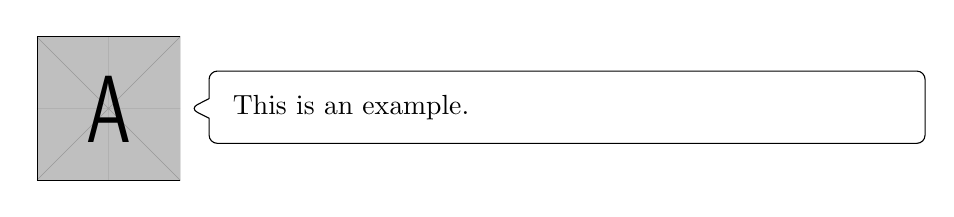
\begin{tikzpicture}
    \node [anchor=south west] at (0, 0) (cartoon) {\includegraphics[width=.15\textwidth,height=.15\textwidth]{example-image-a}};
    \node [anchor=north west,rectangle callout,draw=black,
    callout absolute pointer=(cartoon.east), 
    rounded corners=3pt,text width=0.7\textwidth, inner sep=2ex] at (.19\textwidth,.125\textwidth) {This is an example.};
\end{tikzpicture}}{\thesubsection}
\end{minipage}
&
\begin{minipage}[m]{0.55\textwidth}
\renewcommand\textminus{\mbox{-}}%<<<<<<<<<<<
\begin{lstlisting}[numberstyle=\zebra{red!15}{green!15},numbers=left,basicstyle=\scriptsize] 
\documentclass{article}
\usepackage{tikz}
\usetikzlibrary{shapes.callouts}
 
\begin{document}
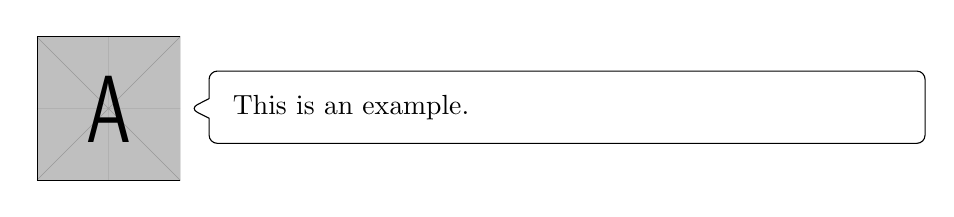
\begin{tikzpicture}
    \node [anchor=south west] at (0, 0) (cartoon) {\includegraphics[width=.15\textwidth,height=.15\textwidth]{example-image-a}};
    \node [anchor=north west,rectangle callout,draw=black,
    callout absolute pointer=(cartoon.east), 
    rounded corners=3pt,text width=0.7\textwidth, inner sep=2ex] at (.19\textwidth,.125\textwidth) {This is an example.};
\end{tikzpicture}
\end{document}
\end{lstlisting}
\end{minipage}
\end{tabular}
\end{table}

%-------------------5.2
\subsection{\hll{Positioning 1 | 2}}
\begin{table}[h!]
\begin{tabular}{c | c}
\begin{minipage}[m]{0.4\textwidth}
\enum{
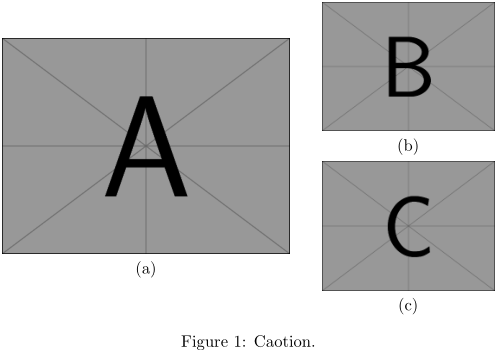
\includegraphics[width=1\linewidth]{5.2.png}}{\thesubsection}
\end{minipage}
&
\begin{minipage}[m]{0.55\textwidth}
\renewcommand\textminus{\mbox{-}}%<<<<<<<<<<<
\begin{lstlisting}[numberstyle=\zebra{red!15}{green!15},numbers=left,basicstyle=\scriptsize]{tex}
\documentclass{article}
\usepackage{graphicx}
\usepackage{subfig}
\begin{document}
\begin{figure}[htp]
\centering
\begin{tabular}{@{}c@{}}
\subfloat{\includegraphics[width=0.5\linewidth]{example-image-a.png}}\\ (a)
\end{tabular}\qquad % some space
\begin{tabular}{@{}c@{}}
\subfloat{\includegraphics[width=0.3\linewidth]{example-image-b.png}}\\ (b)\\[0.1cm]
\subfloat{\includegraphics[width=0.3\linewidth]{example-image-c.png}}\\ (c)
\end{tabular}%\caption{Caption.}
\end{figure}
\end{document}
\end{lstlisting}
\end{minipage}
\end{tabular}
\end{table}


%-------------------5.3
\subsection{\hll{Placing image \xmybox[red!70!white]{anywhere} You want}}
\begin{table}[ht!]
\begin{tabular}{c | c}
\begin{minipage}[m]{0.4\textwidth}
\enum{
 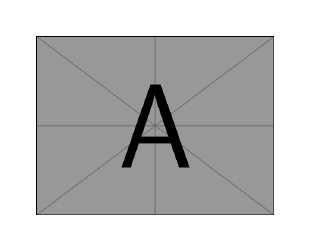
\begin{tikzpicture}
\node[ above left,
      xshift=5cm, %shifting around
      yshift=-3cm]  
{\includegraphics[width=3cm]{example-image-a.png}};
  % define destination coordinates
  \path (5,-3) coordinate (anode);
\end{tikzpicture}}{\thesubsection}

\end{minipage}
&
\begin{minipage}[m]{0.55\textwidth}
\renewcommand\textminus{\mbox{-}}%<<<<<<<<<<<
\begin{lstlisting}[numberstyle=\zebra{red!15}{green!15},numbers=left,basicstyle=\ttfamily\footnotesize]{tex}
\usepackage{graphicx}
\usepackage{tikz}
\begin{document}
\begin{tikzpicture}[overlay, remember picture]
\node[anchor=north west,xshift=4cm,yshift=-11cm]
at (current page.north west) 
{\includegraphics[width=5.5cm]{example-image-a.png}};
\end{tikzpicture}
\end{document}
\end{lstlisting}
\end{minipage}
\end{tabular}
\end{table}




%-------------------5.4
{\subsection{\hll{Italic sabfigure references}}
\begin{table}[h!]
\begin{tabular}{c | c}
\begin{minipage}[m]{0.4\textwidth}
\enum{  \centering
\begin{subfigure}{.25\textwidth}
\centering
\includegraphics[width=.9\linewidth]{example-image-a}
\caption{ \textit{a} }
\label{1a}
\end{subfigure}%
\begin{subfigure}{.25\textwidth}
\centering
\includegraphics[width=.9\linewidth]{example-image-b}
\caption{ \textit{b} }
\label{1b}
\end{subfigure}\\ 

 Fig.  1\textit{a} $\leftarrow$ a in \textbf{\textit{italic}} style
 }{\thesubsection}
\end{minipage}
&
\begin{minipage}[m]{0.55\textwidth}
\renewcommand\textminus{\mbox{-}}%<<<<<<<<<<<
\begin{lstlisting}[numberstyle=\zebra{red!15}{green!15},numbers=left,basicstyle=\ttfamily\scriptsize]{tex}
\documentclass{article}
\usepackage{graphicx}
\usepackage{subcaption}
\renewcommand\thesubfigure{{\itshape\alph{subfigure}}} %<--- added

\begin{document}
\begin{figure}
\centering
\begin{subfigure}{.25\textwidth}
\centering
\includegraphics[width=.6\linewidth]{example-image-a}
\caption{ \textit{a} }\label{1a}
\end{subfigure}%
\begin{subfigure}{.25\textwidth}
\centering
\includegraphics[width=.715\linewidth]{example-image-b}
\caption{ \textit{b} }\label{1b}
\end{subfigure}
\caption{ }\label{fig1}
\end{figure}
 Fig. \ref{1a} $\leftarrow$ a in \textbf{\textit{italic}} style
\end{document}
\end{lstlisting}
\end{minipage}
\end{tabular}
\end{table}}


%-------------------5.5
 
\subsection{\hll{Wrapfigure}}
\begin{table}[h!]
\begin{tabular}{c | c}
\begin{minipage}[m]{0.4\textwidth}
\enum{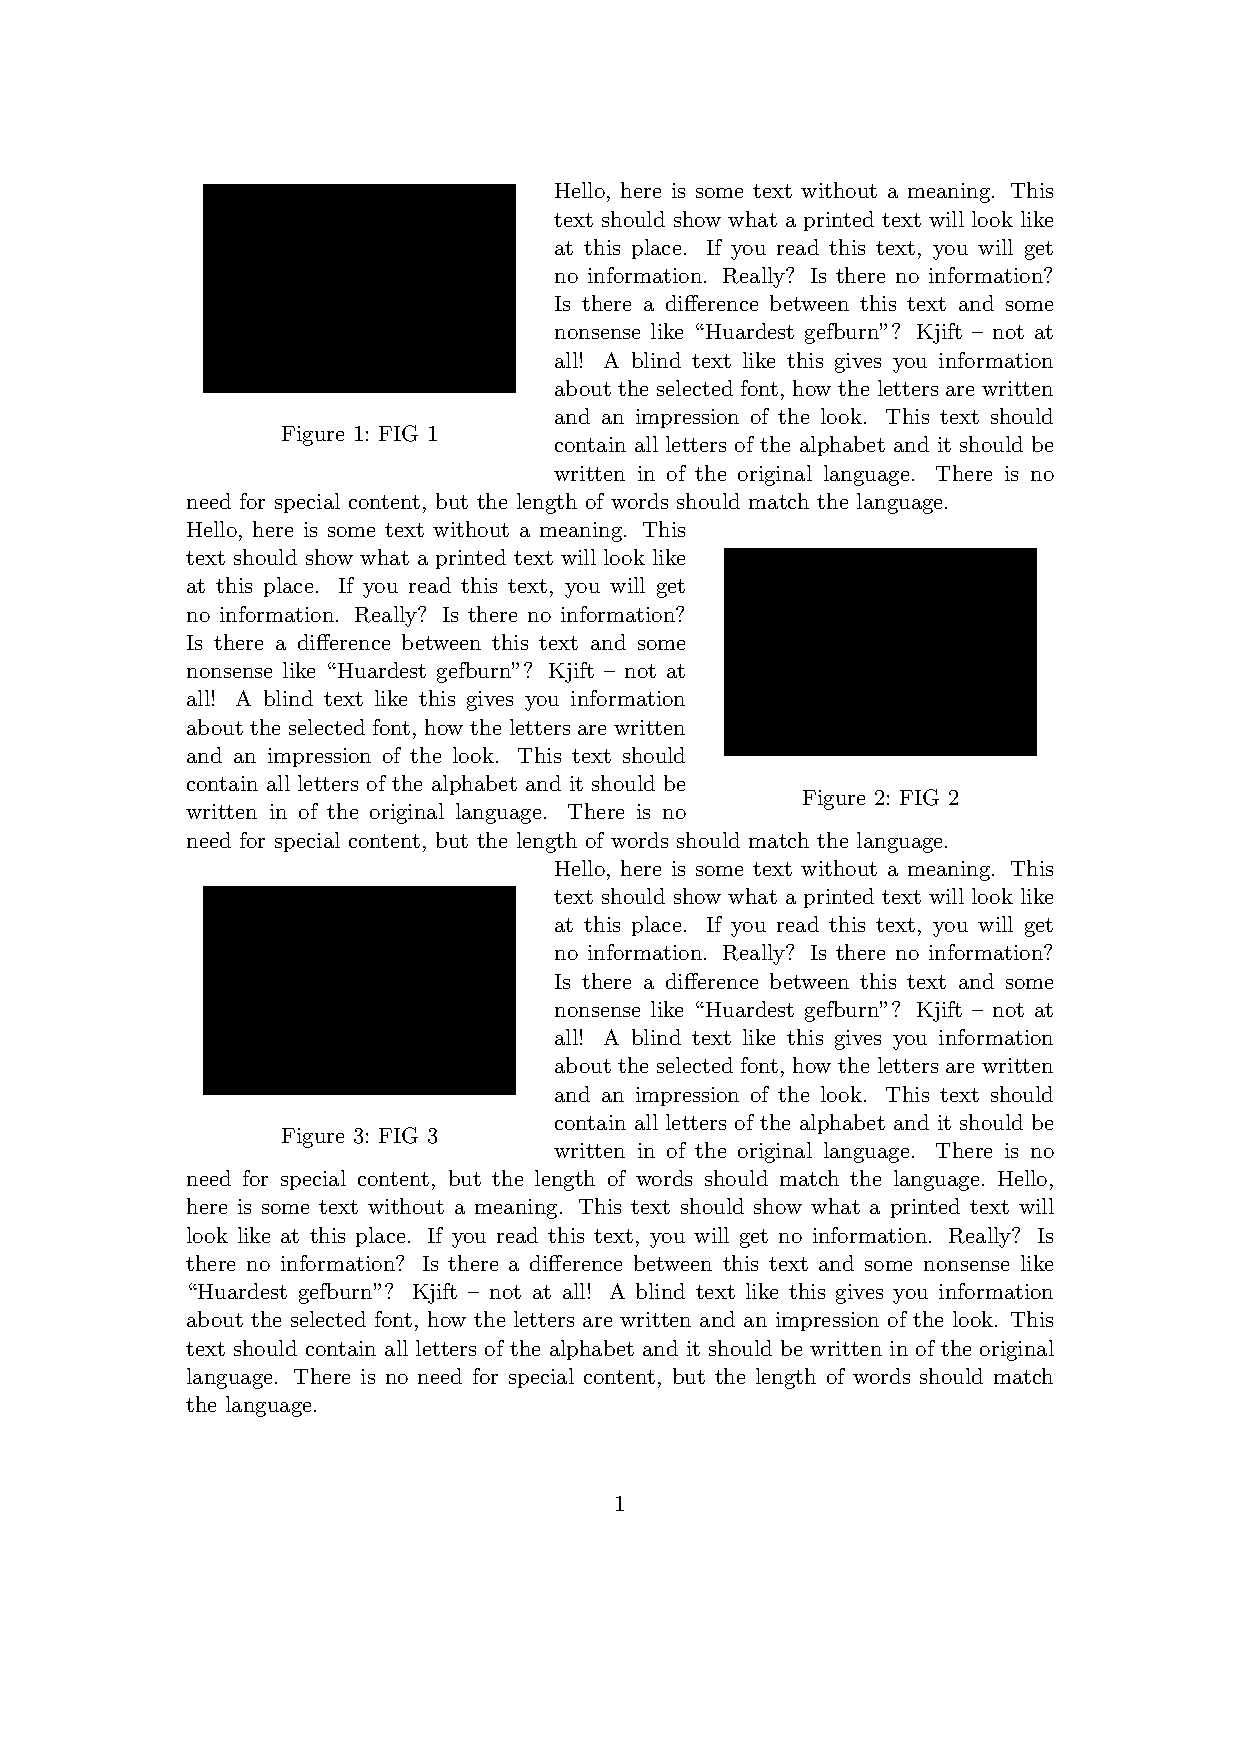
\includegraphics[width=1.1\linewidth]{C:/Users/user/Desktop/eBook/images/5.5/5.5.pdf}}{\thesubsection}
\end{minipage}
&
\begin{minipage}[m]{0.55\textwidth}
\renewcommand\textminus{\mbox{-}}%<<<<<<<<<<<
\begin{lstlisting}[numberstyle=\zebra{red!15}{green!15},numbers=left,basicstyle=\ttfamily\scriptsize]
\documentclass[11pt]{scrartcl}
\usepackage[english]{babel}
\usepackage[utf8]{inputenc}
\usepackage{blindtext}
\usepackage[demo]{graphicx}
\usepackage{wrapfig}
\setlength{\parindent}{0pt}

\begin{document}
\begin{wrapfigure}[11]{l}{0.4\textwidth}
  \centering  
  \includegraphics[scale=0.1]{Bild}
  \caption{FIG 1}
\end{wrapfigure}
\blindtext

\begin{wrapfigure}[11]{r}{0.4\textwidth}
  \centering  
  \includegraphics[scale=0.1]{Bild}
  \caption{FIG 2}
\end{wrapfigure}
\blindtext

\begin{wrapfigure}[11]{l}{0.4\textwidth}
  \centering  
  \includegraphics[scale=0.1]{Bild}
  \caption{FIG 3}
\end{wrapfigure}
\blindtext 
\blindtext 
\end{document}
\end{lstlisting}
\end{minipage}
\end{tabular}
\end{table}
 

 %-------------------5.6
 \subsection{\hll{Figures in landscape mode}}
\begin{table}[h!]
\begin{tabular}{c | c}
\begin{minipage}[m]{0.4\textwidth}
\enum{ 
  \hfill
  \rotatebox{90}{%
    \begin{minipage}{0.45\linewidth}
      \includegraphics[width=\linewidth]{example-image-a}
      \caption{ }
      \label{fig:First}
    \end{minipage}
  }\hfill
  \rotatebox{90}{%
    \begin{minipage}{0.45\linewidth}
      \includegraphics[width=\linewidth]{example-image-b}
      \caption{ }
      \label{fig:Firstt}
    \end{minipage}
  }\hfill\strut}{\thesubsection}
\end{minipage}
&
\begin{minipage}[m]{0.55\textwidth}
\renewcommand\textminus{\mbox{-}}%<<<<<<<<<<<
\begin{lstlisting}[numberstyle=\zebra{red!15}{green!15},numbers=left,basicstyle=\ttfamily\scriptsize]
\documentclass[12pt]{report} 
\usepackage{graphicx}
\usepackage{lipsum}
\begin{document}
qqqqqqq
\begin{figure}[htb]
  \hfill
  \rotatebox{90}{%
    \begin{minipage}{0.45\linewidth}
      \includegraphics[width=\linewidth]{example-image-a}
      \caption{Caption1}
      \label{fig:First}
    \end{minipage}
  }\hfill
  \rotatebox{90}{%
    \begin{minipage}{0.45\linewidth}
      \includegraphics[width=\linewidth]{example-image-b}
      \caption{Caption2}
      \label{fig:First}
    \end{minipage}
  }\hfill\strut
\end{figure}

\end{document}
\end{lstlisting}
\end{minipage}
\end{tabular}
\end{table}

 
 %-------------------5.7
\subsection{\hll{Three figures in a row}}
\begin{table}[h!]
\begin{tabular}{c | c}
\begin{minipage}[m]{0.4\textwidth}
\enum{\centering
\includegraphics[width=1\linewidth]{5.7.png}}{\thesubsection}
\end{minipage}
&
\begin{minipage}[m]{0.55\textwidth}
\renewcommand\textminus{\mbox{-}}%<<<<<<<<<<<
\begin{lstlisting}[numberstyle=\zebra{red!15}{green!15},numbers=left,basicstyle=\ttfamily\scriptsize]
\documentclass[english]{article}
\usepackage[demo]{graphicx}
\usepackage{babel,blindtext}

\begin{document}
\blindtext
\begin{figure}[!htb]
\minipage{0.32\textwidth}
  \includegraphics[width=\linewidth]{delete_gesture.png}
  \caption{Caption}\label{fig:awesome_image1}
\endminipage\hfill
\minipage{0.32\textwidth}
  \includegraphics[width=\linewidth]{ok_gesture.png}
  \caption{Caption}\label{fig:awesome_image2}
\endminipage\hfill
\minipage{0.32\textwidth}%
  \includegraphics[width=\linewidth]{settings_gesture.png}
  \caption{Caption}\label{fig:awesome_image3}
\endminipage
\end{figure}
\blindtext
\end{document}
\end{lstlisting}
\end{minipage}
\end{tabular}
\end{table}
\clearpage

%-------------------5.8
\subsection{\hll{Image as a background in a presentation}}
\begin{table}[h!]
\begin{tabular}{c | c}
\begin{minipage}[m]{0.4\textwidth}
\enum{\centering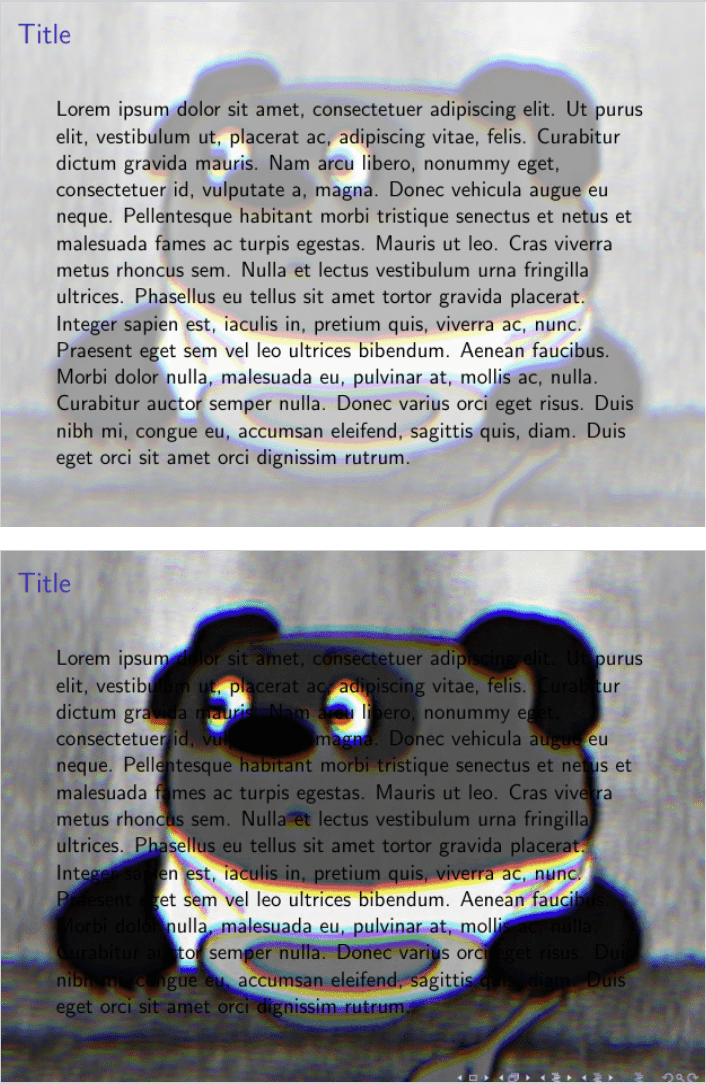
\includegraphics[width=1\linewidth]{5.8.png}}{\thesubsection}
\end{minipage}
&
\begin{minipage}[m]{0.55\textwidth}
\renewcommand\textminus{\mbox{-}}%<<<<<<<<<<<
\begin{lstlisting}[numberstyle=\zebra{red!15}{green!15},numbers=left,basicstyle=\ttfamily\scriptsize]
\documentclass{beamer}
\usepackage{transparent}
\usepackage{lipsum}

\begin{document}
\usebackgroundtemplate{\transparent{0.4}\includegraphics[width=\paperwidth,height=\paperheight]{example-image-a}}
\begin{frame}{Title}
\lipsum[1]
\end{frame}
\usebackgroundtemplate{\includegraphics[width=\paperwidth,height=\paperheight]{example-image-a}}
\begin{frame}{Title}
\lipsum[1]
\end{frame}
\end{document}
\end{lstlisting}
\end{minipage}
\end{tabular}
\end{table}

%-------------------5.9
 
%-------------------5.10
%-------------------5.11

